\documentclass[12pt]{article}
\usepackage[margin=1in]{geometry} 
\usepackage{amsmath}
\usepackage{tcolorbox}
\usepackage{amssymb}
\usepackage{amsthm}
\usepackage{lastpage}
\usepackage{fancyhdr}
\usepackage{accents}
\usepackage{url}
\usepackage[colorlinks]{hyperref}
\usepackage{changepage}
\usepackage{booktabs}
\usepackage[none]{hyphenat}
\usepackage{graphicx}
\usepackage{parskip}
\pagestyle{fancy}
\setlength{\headheight}{40pt}

\newcommand{\indep}{\rotatebox[origin=c]{90}{$\models$}}
\newcommand{\ubar}[1]{\underaccent{\bar}{#1}}

\begin{document}

\lhead{Homework \#1 \\ \textbf{Student name: James Hahn} }
\rhead{CS8803 - PGM \\ Probabilistic Graphical Models} 
\cfoot{\thepage\ of \pageref{LastPage}}
\noindent

\textbf{Problem 1.1}
\begin{enumerate}
	\item \textbf{False.} Active path from Season $\rightarrow$ Flu $\rightarrow$ Chills.
	\item \textbf{True.} All paths are blocked: Flu blocks all possible paths.
	\item \textbf{False.} Active path from Season $\rightarrow$ Dehydration $\rightarrow$ Headache.
	\item \textbf{True.} All paths are blocked: Flu blocks one path and Dehydration blocks the other path.
	\item \textbf{False.} Active path from Season $\rightarrow$ Flu $\rightarrow$ Headache $\rightarrow$ Dizziness $\rightarrow$ Nausea.
	\item \textbf{True.} All paths are blocked: Headache blocks Season $\rightarrow$ Flu $\rightarrow$ Headache $\rightarrow$ Dizziness $\rightarrow$ Nausea, Dehydration blocks Season $\rightarrow$ Dehydration $\rightarrow$ Nausea, and Dehydration blocks Season $\rightarrow$ Dehydration $\rightarrow$ Headache $\rightarrow$ Dizziness $\rightarrow$ Nausea.
	\item \textbf{False.} Active path from Flu $\rightarrow$ Season $\rightarrow$ Dehydration.
	\item \textbf{False.} Since Flu $\rightarrow$ Headache $\leftarrow$ Dehydration is a v-structure and Headache is observed, that path becomes activate, so Flu $\rightarrow$ Headache $\rightarrow$ Dehydration is an active path.
	\item \textbf{True.} All paths are blocked: Season blocks Flu $\rightarrow$ Season $\rightarrow$ Dehydration and Headache, because it's not observed, blocks Flu $\rightarrow$ Headache $\rightarrow$ Dehydration.
	\item \textbf{False.} Active path from Flu $\rightarrow$ Headache $\rightarrow$ Dizziness $\rightarrow$ Nausea $\rightarrow$ Dehydration because Dizziness $\rightarrow$ Nausea $\leftarrow$ Dehydration is a v-structure and Nausea is observed, making it active.
	\item \textbf{False.} Active path from Chills $\rightarrow$ Flu $\rightarrow$ Season $\rightarrow$ Dehydration $\rightarrow$ Nausea.
	\item \textbf{False.} Active path from Chills $\rightarrow$ Flu $\rightarrow$ Season $\rightarrow$ Dehydration $\rightarrow$ Nausea.
\end{enumerate}

\pagebreak\textbf{Problem 1.2}
\begin{enumerate}
	\item \small P(S, F, D, C, H, Z, N) = P(S)P(F $\vert$ S)P(C $\vert$ F)P(D $\vert$ S)P(H $\vert$ F, D)P(Z $\vert$ H)P(N $\vert$ D, Z)
	\item Let K =  $\phi_1(S)\phi_2(F)\phi_3(D)\phi_4(C)\phi_5(H)\phi_6(N)\phi_7(Z)\phi_8(S, F)\phi_9(F, C)\phi_{10}(N, Z)\phi_{11}(F, H)\\\phi_{12}(F, H)\phi_{13}(D, H)\phi_{14}(D, N)\phi_{15}(H, Z)$
	
	The factorized form is $$\frac{K}{\sum_{S, F, D, C, H, N, Z} K}$$ In case it is difficult to read, the denominator is the summation over all random variables with the value in the summation being the value K (a user would just need to substitute the correct values into K for each iteration).
\end{enumerate}

\pagebreak\textbf{Problem 1.3}
\begin{enumerate}
	\item P(F = true)\\
	= $\sum_S$ P(F = true, S = s) \\
	= $\sum_S$ P(F = true $\vert$ S = s)P(S = s) \\
	= P(F = true $\vert$ S = winter)P(S = winter) + P(F = true $\vert$ S
	= summer)P(S = summer) \\
	= 0.4(0.5) + 0.1(0.5) \\
	= 0.2 + 0.05 \\
	= \textbf{0.25} 
	\item P(F = true $\vert$ S = winter) = \textbf{0.4} (it's in the second CPD table)
	\item To aid in solving this problem, I will compute 2 new probabilities given the CPDs:
	
	$P(S = \text{winter} \vert F = \text{true}) = \frac{P(F = \text{true} \vert S = \text{winter})P(S = \text{winter})}{P(F = \text{true})} = \frac{0.4(0.5)}{0.25} = 0.8$
	
	$P(S = \text{winter} \vert F = \text{false}) = \frac{P(F = \text{false} \vert S = \text{winter})P(S = \text{winter})}{P(F = \text{false})} = \frac{0.6(0.5)}{0.75} = 0.4$
	
	So, now we can calculate the final answer as such:
	
	P(F = true $\vert$ S = winter, H = true) \\
	= $\frac{P(S = \text{winter}, H = \text{true} \vert F = \text{true})P(F = \text{true})}{P(S = \text{winter}, H = \text{true})}$\\
	= $\frac{P(H = \text{true} \vert S = \text{winter}, F = \text{true})P(S = \text{winter} \vert F = \text{true})P(F = \text{true})}{\sum_F P(S = \text{winter}, H = \text{true})P(F)}$\\
	= $\frac{P(H = \text{true} \vert D, F = \text{true})P(D \vert S = \text{winter})P(S = \text{winter} \vert F = \text{true})P(F = \text{true})}{\sum_F P(H = \text{true} \vert S = \text{winter})P(S = \text{winter} \vert F = f)P(F = f)}$\\
	= $\frac{\sum_D P(H = \text{true} \vert D = d, F = \text{true})P(D = d \vert S = \text{winter})P(S = \text{winter} \vert F = \text{true})P(F = \text{true})}{\sum_{D, F} P(H = \text{true} \vert D = d, F = f)P(D = d \vert S = \text{winter})P(S = \text{winter} \vert F = f)P(F = f)}$\\
	= $\frac{0.8(0.9)(0.8)(0.25) + 0.9(0.1)(0.8)(0.25)}{0.3(0.9)(0.4)(0.75) + 0.8(0.9)(0.8)(0.25) + 0.8(0.1)(0.4)(0.75) + 0.9(0.1)(0.8)(0.25)}$\\
	= $\frac{0.018 + 0.144}{(0.018 + 0.144) + (0.024 + 0.081)}$\\
	= $\frac{0.162}{0.267}$\\
	= \textbf{0.6067}\\
	\item P(F $\vert$ S = winter, H = true, D = true)\\
	= $\frac{P(H = \text{true} \vert D = \text{true}, F = \text{true})P(D = \text{true} \vert S = \text{winter})P(S = \text{winter} \vert F = \text{true})P(F = \text{true})}{\sum_F P(H = \text{true} \vert D = \text{true}, F = f)P(D = \text{true} \vert S = \text{winter})P(S = \text{winter} \vert F = f)P(F = f)}$\\
	= $\frac{0.9(0.1)(0.8)(0.25)}{0.8(0.1)(0.4)(0.75) + 0.9(0.1)(0.8)(0.25)}$\\
	= $\frac{0.018}{0.024 + 0.018}$\\
	= $\frac{0.018}{0.042}$\\
	= \textbf{0.4286}
	\item Dehydration causes a decrease in your likelihood of having the flu. This is an appropriate conclusion because when we know you are dehydrated, it explains away the effect of the headache on having a flu.
\end{enumerate}

\pagebreak\textbf{Problem 1.4}
\begin{enumerate}
	\item There are no marginal independences in Figure 1 and 2, so no there are no differences.
	\item Yes. In Figure 1, Flu $\indep$ Dehydration $\vert$ Season, but this is not the case in Figure 2 because the trail Flu $\rightarrow$ Headache $\rightarrow$ Dehydration exists.
\end{enumerate}

\pagebreak\textbf{Problem 2.1}
\begin{enumerate}
	\item See the figure drawn below. Please note the slightly shaded in circle ($X_n$).
	
	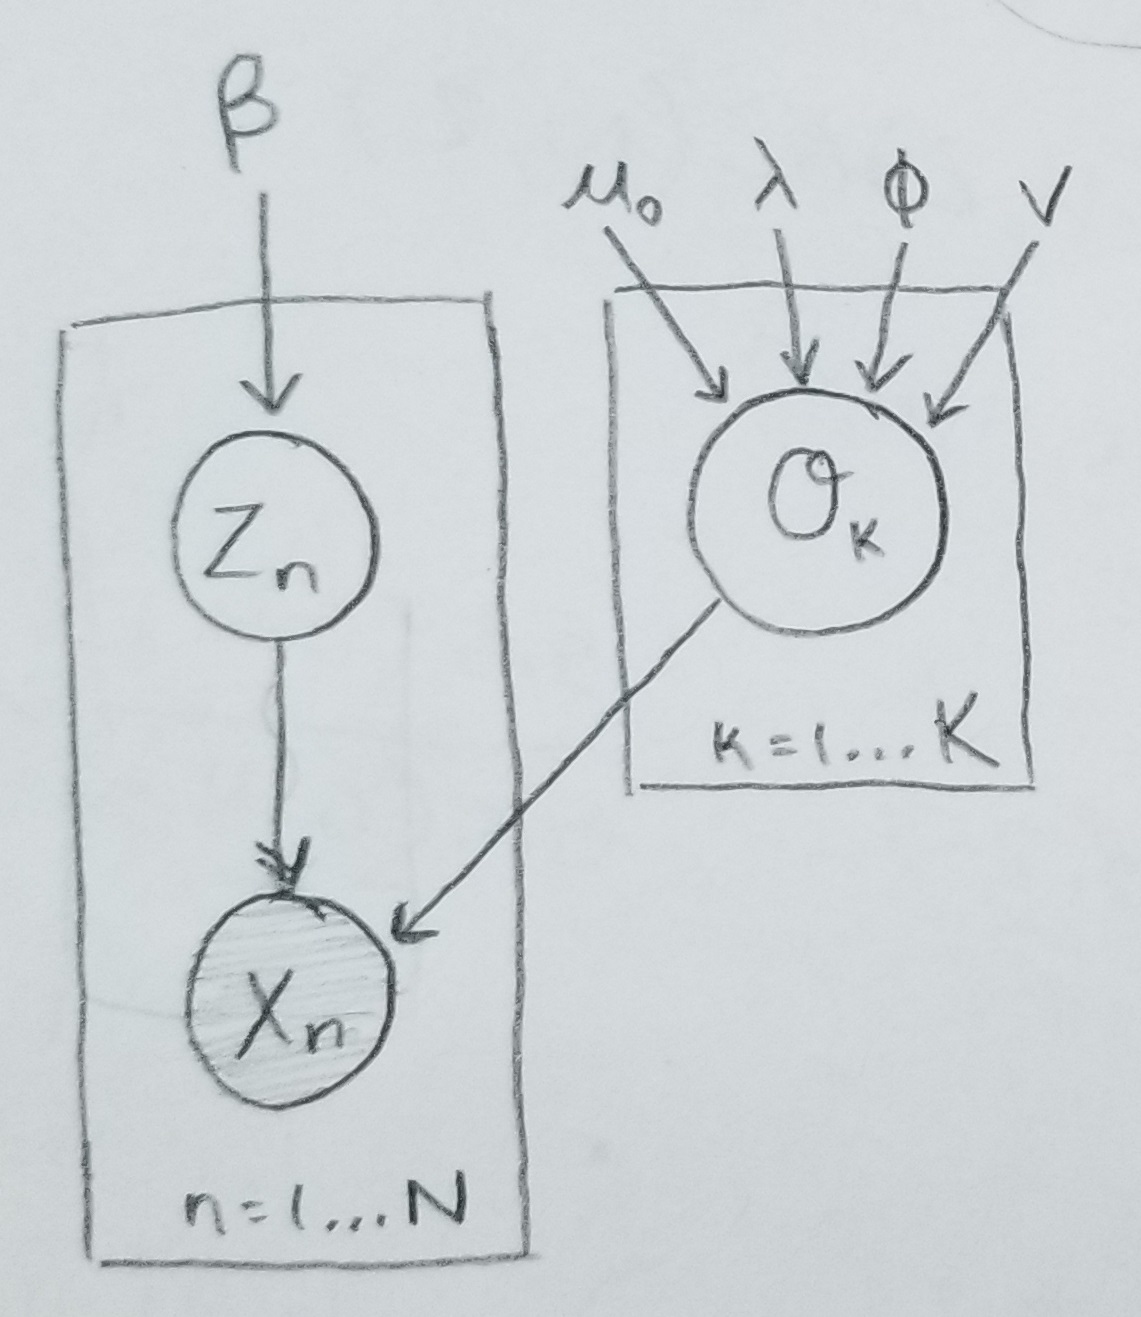
\includegraphics[scale=0.2]{q2-sub1-part1-answer}
	
	\item See the figure drawn below. Please note the slightly shaded in circles ($X_n$ and $Y_n$).
	
	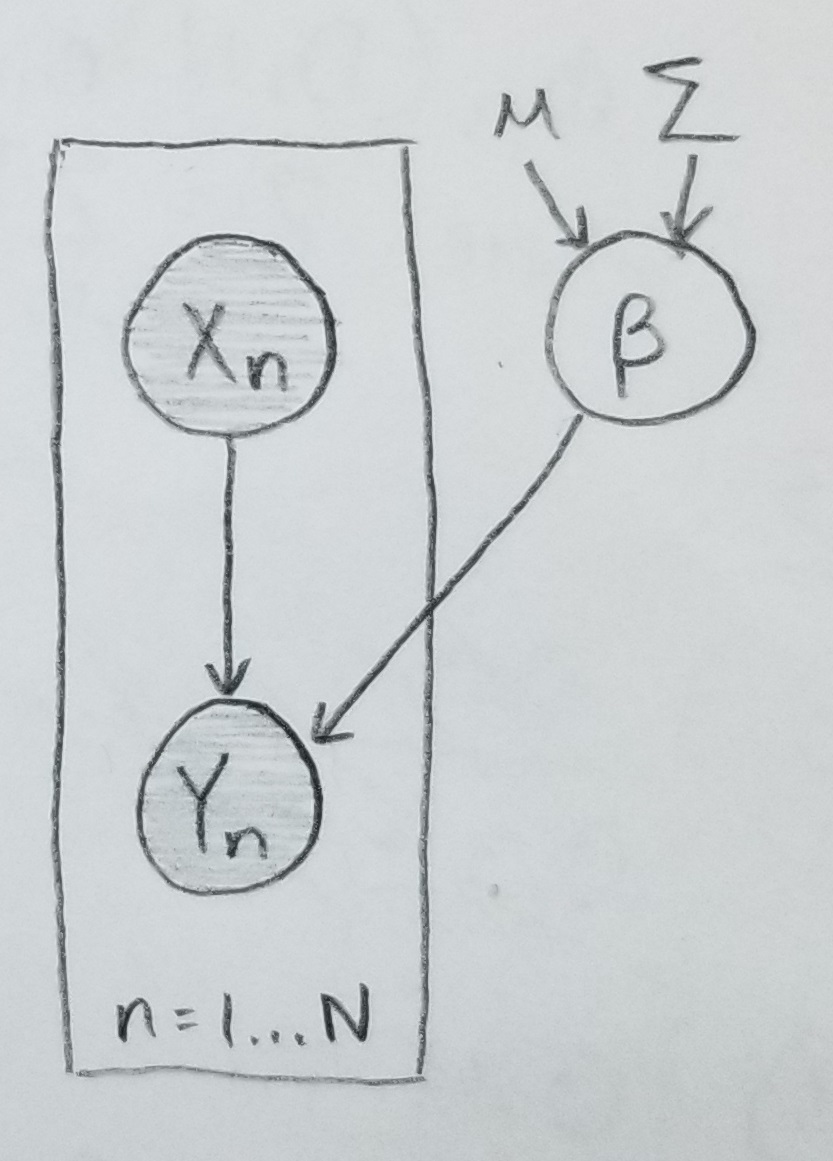
\includegraphics[scale=0.2]{q2-sub1-part2-answer}
\end{enumerate}

\pagebreak\textbf{Problem 2.2}

Let us assume P factorizes according to G.

We know $\textbf{X} = X_i \cup \text{Pa}(X_i) \cup \text{NonDesc}(X_i) \cup \text{Desc}(X_i)$.

From that, we can show the following:

$P(X_i \vert \text{Pa}(X_i), \text{NonDesc}(X_i)) \\$

$= \frac{P(X_i, \text{Pa}(X_i), \text{NonDesc}(X_i))}{\sum_{x \in X_i} P(X_i, \text{Pa}(X_i), \text{NonDesc}(X_i))}\quad$(law of total probability)\\

$= \frac{\sum_{X_m \in \text{Desc}(X_i)}P(X_i, \text{Pa}(X_i), \text{NonDesc}(X_i), X_m)}{\sum_{x \in X_i} P(X_i, \text{Pa}(X_i), \text{NonDesc}(X_i))}\\$

$= \frac{\sum_{X_m \in \text{Desc}(X_i)}\prod_{j=1}^{n} P(X_j \vert \text{Pa}(X_j))}{\sum_{x \in X_i} P(X_i, \text{Pa}(X_i), \text{NonDesc}(X_i))}\quad$ (where n = number of vertices in the graph) \\

$= \frac{\sum_{X_m \in \text{Desc}(X_i)} \big[P(X_i \vert \text{Pa}(X_i))\prod_{X_j \in \text{NonDesc}(X_i)}\prod_{X_k \in \text{Pa}(X_i)} \prod_{X_m \in \text{Desc}(X_i)} P(X_j \vert \text{Pa}(X_j)) P(X_k \vert \text{Pa}(X_k)) P(X_m \vert \text{Pa}(X_m))\big]}{\sum_{x \in X_i} P(X_i, \text{Pa}(X_i), \text{NonDesc}(X_i))}\\$

$= \frac{\sum_{X_m \in \text{Desc}(X_i)} \big[P(X_i \vert \text{Pa}(X_i))\prod_{X_j \in \text{NonDesc}(X_i)} P(X_j \vert \text{Pa}(X_j))\prod_{X_k \in \text{Pa}(X_i)} P(X_k \vert \text{Pa}(X_k))\prod_{X_m \in \text{Desc}(X_i)} P(X_m \vert \text{Pa}(X_m))\big]}{\sum_{x \in X_i} P(X_i, \text{Pa}(X_i), \text{NonDesc}(X_i))}\\$

$= \frac{P(X_i \vert \text{Pa}(X_i))\prod_{X_j \in \text{NonDesc}(X_i)} P(X_j \vert \text{Pa}(X_j))\prod_{X_k \in \text{Pa}(X_i)} P(X_k \vert \text{Pa}(X_k))\sum_{X_m \in \text{Desc}(X_i)}\prod_{X_m \in \text{Desc}(X_i)} P(X_m \vert \text{Pa}(X_m))}{\sum_{x \in X_i} P(X_i, \text{Pa}(X_i), \text{NonDesc}(X_i))}\\$

We know $\sum_{X_m \in \text{Desc}(X_i)}\prod_{X_m \in \text{Desc}(X_i)} P(X_m \vert \text{Pa}(X_m)) = 1$, so this term can be removed from the numerator. We can continue as follows:\\

$= \frac{P(X_i \vert \text{Pa}(X_i))\prod_{X_j \in \text{NonDesc}(X_i)} P(X_j \vert \text{Pa}(X_j))\prod_{X_k \in \text{Pa}(X_i)} P(X_k \vert \text{Pa}(X_k))}{\sum_{x \in X_i} P(X_i, \text{Pa}(X_i), \text{NonDesc}(X_i))}\\$

$= \frac{P(X_i \vert \text{Pa}(X_i))\prod_{X_j \in \text{NonDesc}(X_i)} P(X_j \vert \text{Pa}(X_j))\prod_{X_k \in \text{Pa}(X_i)} P(X_k \vert \text{Pa}(X_k))}{\sum_{x \in X_i} P(X_i \vert \text{Pa}(X_i)) \prod_{X_j \in \text{NonDesc}(X_i)} P(X_j \vert \text{Pa}(X_j)) \prod_{X_k \in \text{Pa}(X_i)} P(X_k \vert \text{Pa}(X_k))}\\$

$= \frac{P(X_i \vert \text{Pa}(X_i))\prod_{X_j \in \text{NonDesc}(X_i)} P(X_j \vert \text{Pa}(X_j))\prod_{X_k \in \text{Pa}(X_i)} P(X_k \vert \text{Pa}(X_k))}{\prod_{X_j \in \text{NonDesc}(X_i)} P(X_j \vert \text{Pa}(X_j)) \prod_{X_k \in \text{Pa}(X_i)} P(X_k \vert \text{Pa}(X_k))}\quad$\scalebox{1}{(since $\sum_{x \in X_i} P(X_i \vert \text{Pa}(X_i)) = 1$)}\\

$= P(X_i \vert \text{Pa}(X_i))$ \\

So, we have shown $P(X_i \vert \text{Pa}(X_i), \text{NonDesc}(X_i)) = P(X_i \vert \text{Pa}(X_i))$.

This means $X_i$ $\indep$ $\text{NonDesc}(X_i)$ $\vert$ $\text{Pa}(X_i)$.

$\therefore$ G is an I-map of P $\qed$

\pagebreak\textbf{Problem 2.3}

We want to show $\text{d-sep}_G(X; Y \vert Z)$ iff $\text{sep}_H(X; Y \vert Z)$.

First, we will show $\text{d-sep}_G(X; Y \vert Z) \implies \text{sep}_H(X; Y \vert Z)$.

Let us assume $\text{d-sep}_G(X; Y \vert Z)$.

Because of $\text{d-sep}_G(X; Y \vert Z)$, there is no active trail between any node $x\in X$ and $y\in Y$ given Z. In other words, all trails between X and Y are inactive given Z.

By the definition of an active trail in a Bayesian network, it must satisfy both of the following conditions: (1) For all V structures $m_{i-1} \rightarrow m_i \leftarrow m_{i+1}$, then $m_i\in Z$ or $\text{Desc}(m_i)\in Z$, (2) no other node in the trail exists in Z. Since all trails are inactive, all trails must violate one of the two conditions above. 

As such, for each trail $T : M_i \rightarrow \dots \rightarrow M_n$ there are two cases:
\begin{enumerate}
	\item T violates condition 1, which means for a given V structure $m_{j-1} \rightarrow m_j \leftarrow m_{j+1}$, we have $m_j, \text{Desc}(m_j)\notin Z$. Let $P = m_j \cup \text{Desc}(m_j)$. Since $m_j$ and its descendants are not observed, we have $P \notin U \cup \text{Ancestors}_U \implies P \notin H$. As such, that V-structure, which consists solely of inactive nodes already, is nonexistent in H, so it is an inactive trail in H by definition.
	\item T violates condition 2, which means there exists at least one observed node $m_j$. In this case, this exact trail is inactive by definition in the Markov network H anyway.
\end{enumerate}

$\therefore$ We have shown $\text{d-sep}_G(X; Y \vert Z) \implies \text{sep}_H(X; Y \vert Z)$.

Now, we will show $\text{sep}_H(X; Y \vert Z) \implies \text{d-sep}_G(X; Y \vert Z)$.

Let us assume $\text{sep}_H(X; Y \vert Z)$.

Because of $\text{sep}_H(X; Y \vert Z)$, there is no active trail between any node $x\in X$ and $y\in Y$ given Z. This means all trails between X and Y are inactive given Z.

By the definition of an active trail in a Markov network, it must satisfy one condition: (1) for all nodes in the trail, no node exists in Z. Since all trails are inactive, they all break this condition. There are three necessary cases to show:

\begin{enumerate}
	\item Moralized parents in H (corresponding to an existing V structure in G): Two parents ($m_{i-1}, m_{i+1}$) in a V structure $m_{i-1} \rightarrow m_j \leftarrow m_{i+1}$ are moralized in H. Since the parents are moralized, this means $m_j\in Z$ or $\text{Desc}(m_j)\in Z$, so this V structure is active in G. As such, the moralized parents create a mini active trail in H (i.e. $m_{i-1}$ --- $m_{i+1}$ exists), following the precedent that that V structure is active in G due to the presence of an observed $m_j$ or descendant of $m_j$. So, these moralized parents, which produce an active trail in H, represent an active trail in G. (i.e. every active path involving moralized parents in H indicates an active V-structure in G)
	\item Non-moralized parents in H (corresponding to an existing V structure in G): Two parents ($m_{i-1}, m_{i+1}$) in a V structure $m_{i-1} \rightarrow m_j \leftarrow m_{i+1}$ are non-moralized in H. Since the two parents are not moralized, this means $m_j, \text{Desc}(m_j)\notin Z$, which means that V structure is not active in G (otherwise, $m_j$ or Desc($m_j$) would be observed, which means it is active V-structure in G AND they would be in $U \cup \text{Ancestors}_U = H$). So, since $m_j, \text{Desc}(m_j)\notin Z$, there is no direct path in H between the parents \\(i.e. $m_{i-1}$ --- $m_{i+1}$ does not exist), which as shown above, implies that V structure is inactive in G. This indicates this inactive path is inactive in G. (i.e. every pair of non-moralized parents in H indicates an inactive V-structure in G)
	\item Three-node trail (corresponding to a causal/evidential trail or common cause in G): $m_i\in Z$ exists on a trail $T \in H$ (i.e. $T$ is inactive in H), so $T$ is inactive in G due to the definition of a casual/evidential trail or common cause. Similarly, if $m_i\notin Z$, then that three-node trail is active, similarly to how it would be in G. (i.e. every inactive three-node trail in H indicates an inactive three-node trail in G)
\end{enumerate}

From the three cases above, we can see moralized parents in H create an active mini-trail between two parents of a V-structure and indicates an active V-structure in G, non-moralized parents in H does not create a mini-trail between two parents of a V-structure and indicates an inactive V-structure in G, and an inactive three-node trail in H indicates an inactive three-node trail (causal/evidential trail or common cause) in G.

$\therefore$ We have shown $\text{sep}_H(X; Y \vert Z) \implies \text{d-sep}_G(X; Y \vert Z)$.

$\therefore$ We have shown both directions and $\text{d-sep}_G(X; Y \vert Z)$ iff $\text{sep}_H(X; Y \vert Z). \quad\qed$

\pagebreak\textbf{Problem 2.4}

The joint distribution for the non-marginalized bayesian network is as follows:

P(B, E, T, N, J, M, A) = P(B)P(E)P(T)P(N)P(A $\vert$ B, E)P(J $\vert$ A, T)P(M $\vert$ A, N)

We want to calculate the marginalized distribution P(B, E, T, N, J, M).

(*) Since we are marginalizing over A, we know P(A $\vert$ B, E) = 1.

Now, we know, a marginalized joint distribution over some variable $x_n$ means $P(x_1, \dots, x_n) = P(x_1, \dots, x_{n-1})$. Using this rule, we can infer the following:

(@) $P(J \vert A, T) = \frac{P(J, A, T)}{P(A, T)} = \frac{P(J, T)}{P(T)} = P(J \vert T)$

(\#) $P(M \vert A, N) = \frac{P(M, A, N)}{P(A, N)} = \frac{P(M, N)}{P(N)} = P(M \vert N)$

As such, using (*), (@), and (\#), we can reduce the joint distribution to the marginalized distribution to get:

P(B, E, T, N, J, M) = P(B)P(E)P(T)P(N)P(J $\vert$ T)P(M $\vert$ N)

So, with this new joint distribution after marginalizing over A (Alarm) in the original joint distribution, we can see the only dependencies are (J, T) and (M, N). The resultant bayesian network showing this minimal I-map is as follows:

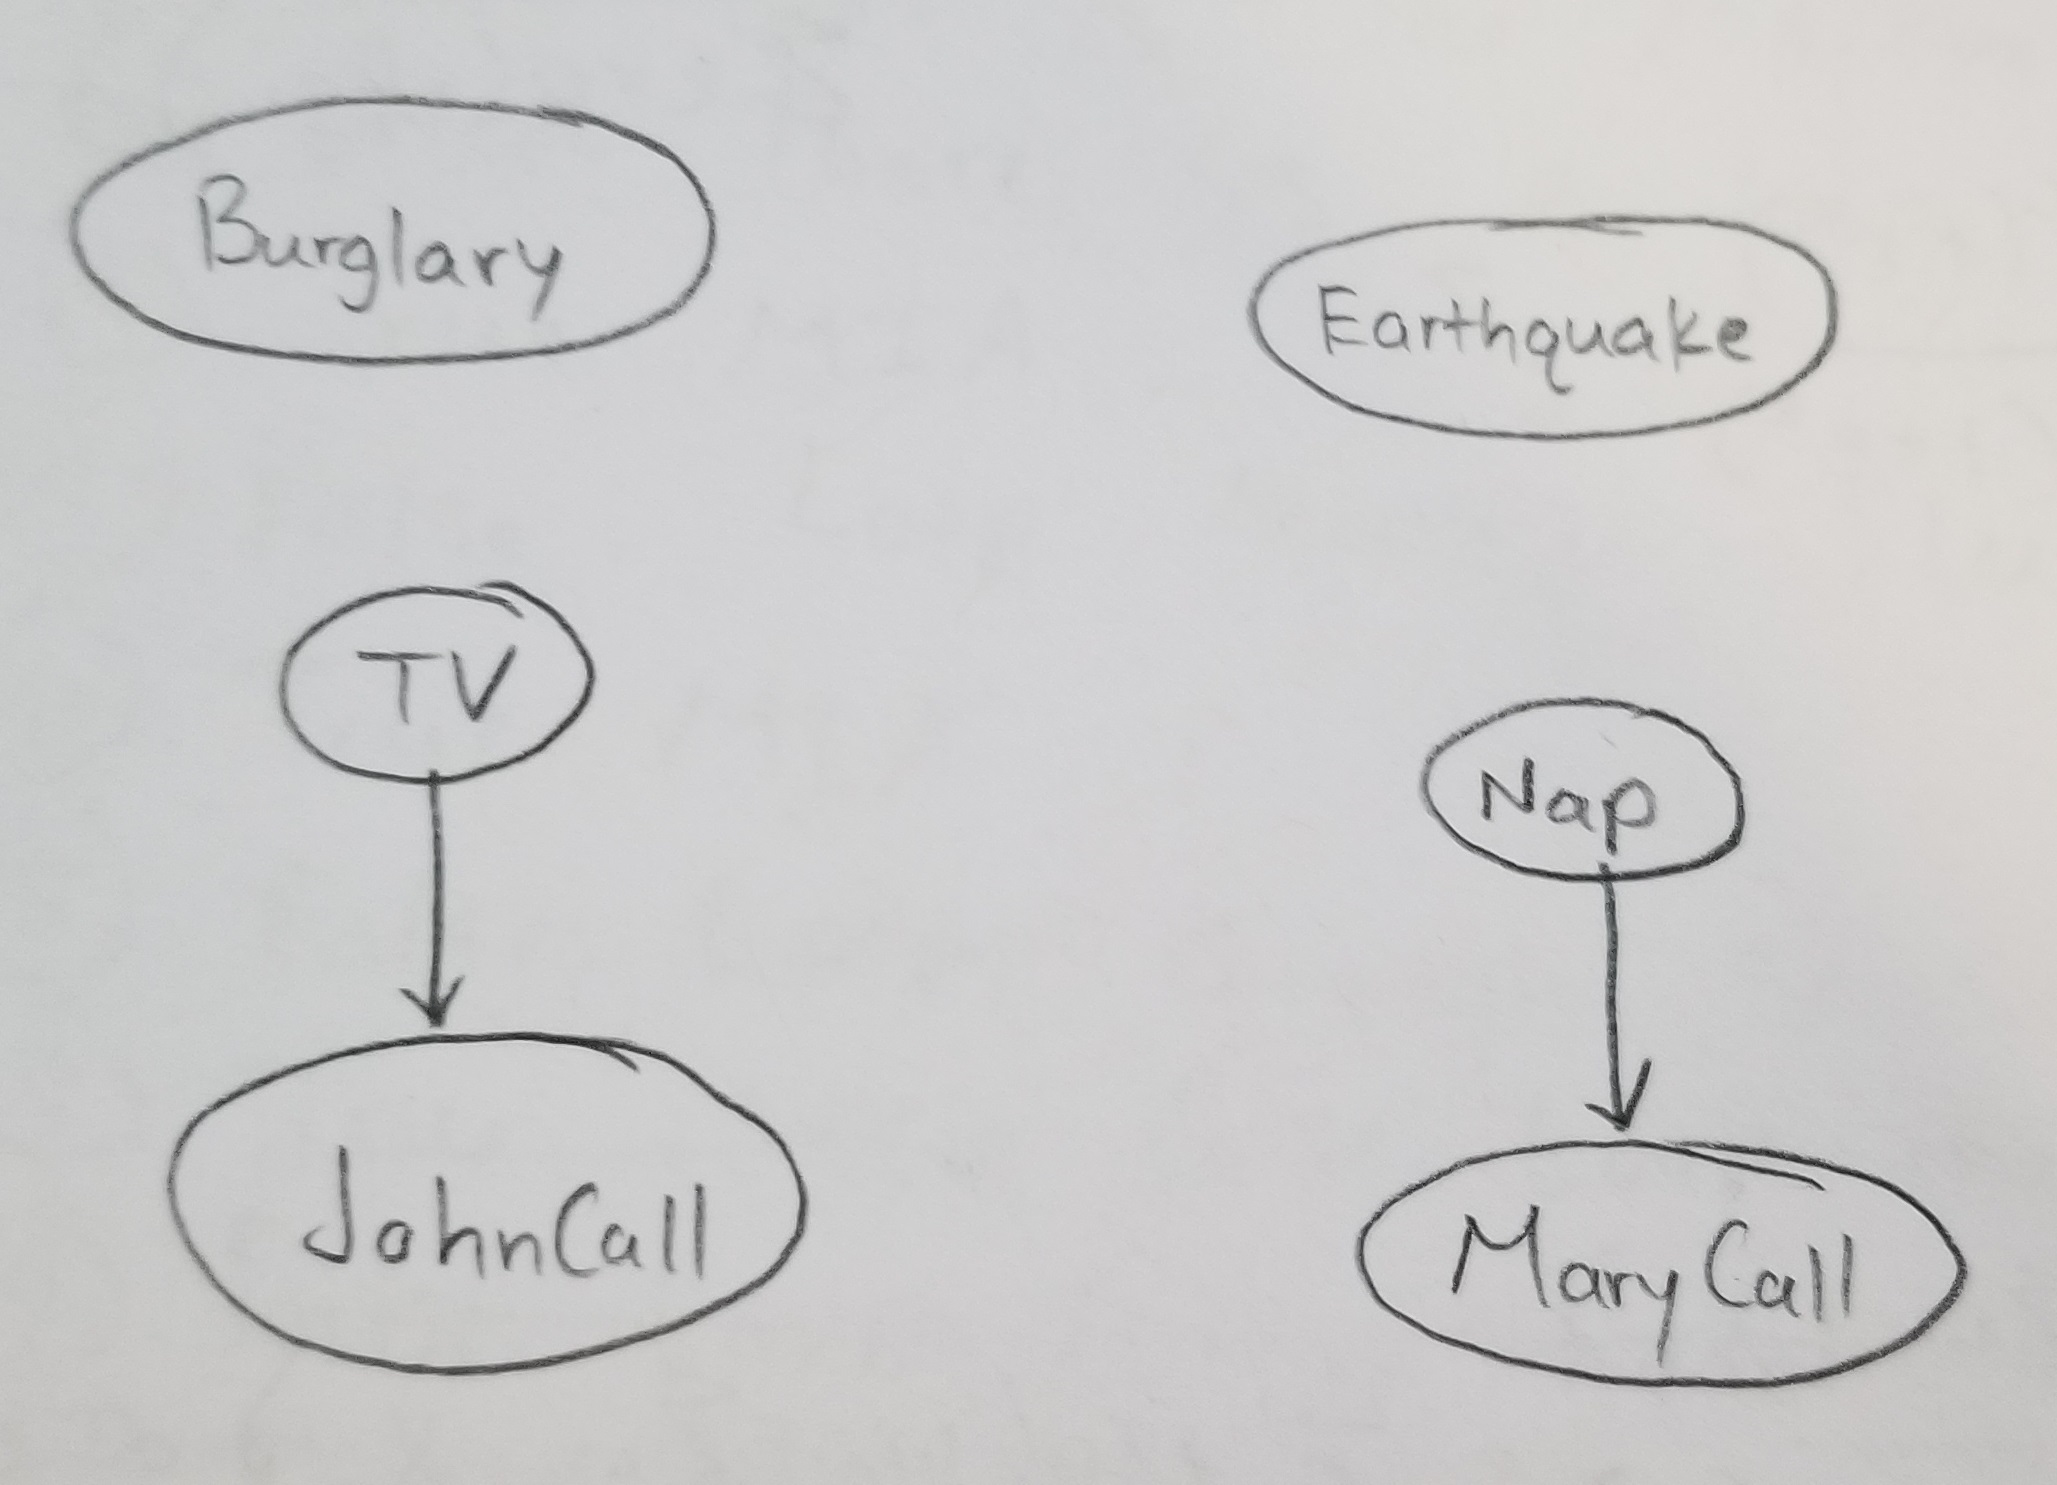
\includegraphics[scale=0.2]{q2-sub3}

\pagebreak\textbf{Problem 2.5}

First, we will show I satisfies strong union ($X \indep Y \vert Z \implies X \indep Y \vert Z, W$).

Assume $X \indep Y \vert Z$.

Since $X \indep Y \vert Z$, all trails $X \rightarrow \dots \rightarrow Y$ are blocked by an observed variable $z \in Z$ in a given three-node structure.

So, observing W will only block additional three-node structures, keeping all independences intact.

$\therefore$ I satisfies strong union.

Next, we will show I satisfies transitivity [$\neg(X \indep A \vert Z) \& \neg(A \indep Y \vert Z) \implies \neg(X \indep Y \vert Z)$].

Assume X depends on A ($\neg(X \indep A \vert Z)$) and A depends on Y ($\neg(A \indep Y \vert Z)$).

Since X depends on A (correlated), there exists trail $T_1$ such that $T_1 : X \rightarrow \dots \rightarrow A$ is active (no node on $T_1$ is observed).

Since A depends on Y (correlated), there exists trail $T_2$ such that $T_2 : A \rightarrow \dots \rightarrow Y$ is active (no node on $T_2$ is observed).

So, we can form a new path $T_3 : X \rightarrow \dots \rightarrow A \rightarrow \dots \rightarrow Y$ such that no node on $T_3$ is observed.

Since no node on $T_3$ is observed, that path is active.

So, since $T_3$ is active, we can simplify $T_3$ such that $T_3 : X \rightarrow \dots \rightarrow Y$, which is the same active path already defined above with simplified notation.

Finally, since there is an active path between X and Y, then X and Y are correlated ($\neg(X \indep Y \vert Z)$).

We have shown $\neg(X \indep A \vert Z) \& \neg(A \indep Y \vert Z) \implies \neg(X \indep Y \vert Z)$. 

$\therefore$ I satisfies transitivity.

$\therefore$ We have shown I satisfies both strong union and transitivity. $\qed$

\pagebreak\textbf{Problem 3}
\begin{enumerate}
	\item First, let us define a logistic regression model as having the form $\frac{\exp(Z)}{\exp(Z) + 1}$.
	
	Let $P(X_i = 0, X_{-i} ; \theta) \propto \exp\{\sum_{s\in V}\theta_s X_s + \sum_{(s, t) \in E} \theta_{s, t} X_s X_t\} = \exp\{0\} = 1$.
	
	Let $P(X_i = 1, X_{-i} ; \theta) \propto \exp\{\sum_{s\in V}\theta_s X_s + \sum_{(s, t) \in E} \theta_{s, t} X_s X_t\} \\
	= \exp\{\sum_{s\in V}\theta_s + \sum_{(i, t) \in E} \theta_{i, t} X_t\}$.
	
	Now, by the law of total probability, we get the following:
	
	$P(X_i = 1 \vert X_{-i} ; \theta) \propto \frac{P(X_i = 1, X_{-i})}{P(X_i = 1, X_{-i}) + P(X_i = 0, X_{-i})}\\
	= \frac{\exp\{\sum_{s\in V}\theta_s + \sum_{(i, t) \in E} \theta_{i, t} X_t\}}{\exp\{\sum_{s\in V}\theta_s + \sum_{(i, t) \in E} \theta_{i, t} X_t\} + 1}$
	
	If we let $Z = \exp\{\sum_{s\in V}\theta_s + \sum_{(i, t) \in E} \theta_{i, t} X_t\}$, we see $P(X_i = 1 \vert X_{-i} ; \theta) \propto \frac{\exp(Z)}{\exp(Z) + 1}$, which is the exact equation representing the logistic regression model as defined above.
	
	$\therefore$ The conditional distribution is given by a logistic regression model. $\qed$
	
	\item The log likelihood  of the probability distribution is as follows:
	
	$P(X \vert W; \theta, \beta) = \exp\Bigg\{\sum_{s\in V} \theta_sX_s + \sum_{(s, t)\in E} \theta_{s, t}X_sX_t + \sum_{s\in V, u\in [q]} \beta_{su}X_sW_u \Bigg\} / Z(W, \theta, \beta)$\\
	$\implies \log P(X \vert W; \theta, \beta) = \log \exp\Bigg\{\sum_{s\in V} \theta_sX_s + \sum_{(s, t)\in E} \theta_{s, t}X_sX_t + \sum_{s\in V, u\in [q]} \beta_{su}X_sW_u \Bigg\} / Z(W, \theta, \beta)$\\
	$\implies \log P(X \vert W; \theta, \beta) = \sum_{s\in V} \theta_sX_s + \sum_{(s, t)\in E} \theta_{s, t}X_sX_t + \sum_{s\in V, u\in [q]} \beta_{su}X_sW_u - \log Z(W, \theta, \beta)$
	
	Now, to calculate the gradients:
	
	$\frac{\delta}{\delta\theta_s}\log P(X \vert W; \theta, \beta) = X_s - \frac{Z'(W, \theta, \beta)}{Z(W, \theta, \beta)}$\\
	$= X_s - \frac{\sum_{X}X_s\exp\Big\{\sum_{s\in V} \theta_sX_s + \sum_{(s, t)\in E} \theta_{s, t}X_sX_t + \sum_{s\in V, u\in [q]} \beta_{su}X_sW_u\Big\}}{Z(W, \theta, \beta)}$\\
	$= X_s - \sum_{X}X_s\exp\Big\{\sum_{s\in V} \theta_sX_s + \sum_{(s, t)\in E} \theta_{s, t}X_sX_t + \sum_{s\in V, u\in [q]} \beta_{su}X_sW_u\Big\}/Z(W, \theta, \beta)$\\
	$= X_s - \sum_{X}X_s P(X \vert W, \theta, \beta)$\\
	$= X_s - E[X_s]$
	
	$\frac{\delta}{\delta\theta_{s, t}}\log P(X \vert W; \theta, \beta) = X_sX_t - \frac{Z'(W, \theta, \beta)}{Z(W, \theta, \beta)}$\\
	$= X_sX_t - \frac{\sum_{X}X_sX_t\exp\Big\{\sum_{s\in V} \theta_sX_s + \sum_{(s, t)\in E} \theta_{s, t}X_sX_t + \sum_{s\in V, u\in [q]} \beta_{su}X_sW_u\Big\}}{Z(W, \theta, \beta)}$\\
	$= X_sX_t - \sum_{X}X_sX_t\exp\Big\{\sum_{s\in V} \theta_sX_s + \sum_{(s, t)\in E} \theta_{s, t}X_sX_t + \sum_{s\in V, u\in [q]} \beta_{su}X_sW_u\Big\}/Z(W, \theta, \beta)$\\
	$= X_sX_t - \sum_{X}X_sX_t P(X \vert W, \theta, \beta)$\\
	$= X_sX_t - E[X_sX_t]$
	
	$\frac{\delta}{\delta\beta_{su}}\log P(X \vert W; \theta, \beta) = X_sW_u - \frac{Z'(W, \theta, \beta)}{Z(W, \theta, \beta)}$\\
	$= X_sW_u - \frac{\sum_{X}X_sW_u\exp\Big\{\sum_{s\in V} \theta_sX_s + \sum_{(s, t)\in E} \theta_{s, t}X_sX_t + \sum_{s\in V, u\in [q]} \beta_{su}X_sW_u\Big\}}{Z(W, \theta, \beta)}$\\
	$= X_sW_u - \sum_{X}X_sW_u\exp\Big\{\sum_{s\in V} \theta_sX_s + \sum_{(s, t)\in E} \theta_{s, t}X_sX_t + \sum_{s\in V, u\in [q]} \beta_{su}X_sW_u\Big\}/Z(W, \theta, \beta)$\\
	$= X_sW_u - \sum_{X}X_sW_u P(X \vert W, \theta, \beta)$\\
	$= X_sW_u - W_uE[X_s]$\\
\end{enumerate}

\pagebreak\textbf{Problem 4}
\begin{enumerate}
	\item \textbf{NOTE:} All code is developed in Python3, so make sure that is installed with the ``python3'' executable readily available. Other than that, no other dependencies are required. You can run this section of the code by running the following commands in order:
	
	1) Extract hmm\_data.zip and navigate to the root directory.
	
	2) python3 rare\_replace.py gene.train gene.train.rare
	
	3) python3 count\_freqs.py gene.train.rare $>$ gene.train.rare.counts
	
	4) python3 hmm.py baseline gene.train.rare.counts gene.test gene\_test.p1.out
	
	5) python3 eval\_gene\_gene\_tagger.py gene.key gene\_test.p1.out
	
	The output from the results/evaluation program can be seen below:
	
	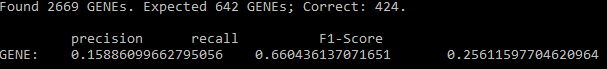
\includegraphics[]{baseline_results}
	
	\item \textbf{NOTE:} This part assumes you have already extracted the hmm\_data.zip file and ran through the steps to evaluate the baseline model. The trigram HMM can be ran and evaluated by running the following commands:
	
	1) python3 hmm.py trigram gene.train.rare.counts gene.test gene\_test.p2.out
	
	2) python3 eval\_gene\_tagger.py gene.key gene\_test.p2.out
	
	The output from the results/evaluation program can be seen below:
	
	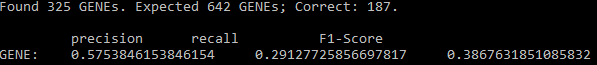
\includegraphics[]{trigram_results}
\end{enumerate}

\pagebreak\textbf{Problem 5}

The joint distribution can be represented as:

$P(x_1, x_2, x_3, x_4, x_5) \\$

$= P(x_1 \vert x_2, x_3, x_4, x_5)P(x_2, x_3, x_4, x_5)$\\

$= P(x_1 \vert x_2, x_5)P(x_2, x_3, x_4, x_5)\\$

$= \frac{P(x_1, x_2, x_5)}{P(x_2, x_5)}P(x_2, x_3, x_4, x_5)$\\

$= \frac{P(x_1, x_2, x_5)}{P(x_2, x_5)}P(x_3 \vert x_2, x_4, x_5)P(x_2, x_4, x_5)$\\

$= \frac{P(x_1, x_2, x_5)}{P(x_2, x_5)}P(x_3 \vert x_2, x_4)P(x_2, x_4, x_5)$\\

$= \frac{P(x_1, x_2, x_5)}{P(x_2, x_5)}\frac{P(x_2, x_3, x_4)}{P(x_2, x_4)}P(x_2, x_4, x_5)\\$

$= \frac{P(x_1, x_2, x_5)P(x_2, x_4, x_5)P(x_2, x_3, x_4)}{P(x_2, x_5)P(x_2, x_4)}\qed\\$

The probability distribution can then be written as:

$P(x_1, x_2, x_3, x_4, x_5) = \frac{\phi(x_1, x_2)\phi(x_2, x_3)\phi(x_3, x_4)\phi(x_4, x_5)\phi(x_1, x_5)}{\sum_{x_1, x_2, x_3, x_4, x_5} \phi(x_1, x_2)\phi(x_2, x_3)\phi(x_3, x_4)\phi(x_4, x_5)\phi(x_1, x_5)}$

We will try to reach this above factorization by marginalizing each distribution term in the numerator and denominator of the following joint distribution given to us:

$P(x_1, x_2, x_3, x_4, x_5) = \frac{P(x_1, x_2, x_5)P(x_2, x_4, x_5)P(x_2, x_3, x_4)}{P(x_2, x_5)P(x_2, x_4)}$

We know the following factorizations of the marginal distributions exist below:

Let $Z = \sum_{x_1, x_2, x_3, x_4, x_5} \phi(x_1, x_2)\phi(x_2, x_3)\phi(x_3, x_4)\phi(x_4, x_5)\phi(x_1, x_5)$

$P(x_1, x_2, x_5) = \frac{\sum_{x_3, x_4} \phi(x_1, x_2)\phi(x_2, x_3)\phi(x_3, x_4)\phi(x_4, x_5)\phi(x_1, x_5)}{Z}$

$P(x_2, x_4, x_5) = \frac{\sum_{x_1, x_3} \phi(x_1, x_2)\phi(x_2, x_3)\phi(x_3, x_4)\phi(x_4, x_5)\phi(x_1, x_5)}{Z}$

$P(x_2, x_3, x_4) = \frac{\sum_{x_1, x_5} \phi(x_1, x_2)\phi(x_2, x_3)\phi(x_3, x_4)\phi(x_4, x_5)\phi(x_1, x_5)}{Z}$

$P(x_2, x_5) = \frac{\sum_{x_1, x_3, x_4} \phi(x_1, x_2)\phi(x_2, x_3)\phi(x_3, x_4)\phi(x_4, x_5)\phi(x_1, x_5)}{Z}$

$P(x_2, x_4) = \frac{\sum_{x_1, x_3, x_5} \phi(x_1, x_2)\phi(x_2, x_3)\phi(x_3, x_4)\phi(x_4, x_5)\phi(x_1, x_5)}{Z}$

Then we can combine them such that:

$P(x_1, x_2, x_3, x_4, x_5)$

$= \frac{P(x_1, x_2, x_5)P(x_2, x_4, x_5)P(x_2, x_3, x_4)}{P(x_2, x_5)P(x_2, x_4)}$

\tiny$= \frac{\frac{1}{Z}\sum_{x_3, x_4} \phi(x_1, x_2)\phi(x_2, x_3)\phi(x_3, x_4)\phi(x_4, x_5)\phi(x_1, x_5)\frac{1}{Z}\sum_{x_1, x_3} \phi(x_1, x_2)\phi(x_2, x_3)\phi(x_3, x_4)\phi(x_4, x_5)\phi(x_1, x_5)\frac{1}{Z}\sum_{x_1, x_5} \phi(x_1, x_2)\phi(x_2, x_3)\phi(x_3, x_4)\phi(x_4, x_5)\phi(x_1, x_5)}{\frac{1}{Z}\sum_{x_1, x_3, x_4} \phi(x_1, x_2)\phi(x_2, x_3)\phi(x_3, x_4)\phi(x_4, x_5)\phi(x_1, x_5)\frac{1}{Z}\sum_{x_1, x_3, x_5} \phi(x_1, x_2)\phi(x_2, x_3)\phi(x_3, x_4)\phi(x_4, x_5)\phi(x_1, x_5)}$

\tiny$= \frac{\frac{1}{Z}\sum_{x_3, x_4} \phi(x_1, x_2)\phi(x_2, x_3)\phi(x_3, x_4)\phi(x_4, x_5)\phi(x_1, x_5)\sum_{x_1, x_3} \phi(x_1, x_2)\phi(x_2, x_3)\phi(x_3, x_4)\phi(x_4, x_5)\phi(x_1, x_5)\sum_{x_1, x_5} \phi(x_1, x_2)\phi(x_2, x_3)\phi(x_3, x_4)\phi(x_4, x_5)\phi(x_1, x_5)}{\sum_{x_1, x_3, x_4} \phi(x_1, x_2)\phi(x_2, x_3)\phi(x_3, x_4)\phi(x_4, x_5)\phi(x_1, x_5)\sum_{x_1, x_3, x_5} \phi(x_1, x_2)\phi(x_2, x_3)\phi(x_3, x_4)\phi(x_4, x_5)\phi(x_1, x_5)}$

\tiny$= \frac{\frac{1}{Z}\phi(x_1, x_2)\phi(x_1, x_5)\phi(x_4, x_5)\phi(x_2, x_3)\phi(x_3, x_4)\sum_{x_3, x_4} \phi(x_2, x_3)\phi(x_3, x_4)\phi(x_4, x_5)\sum_{x_1, x_3} \phi(x_1, x_2)\phi(x_2, x_3)\phi(x_3, x_4)\phi(x_1, x_5)\sum_{x_1, x_5} \phi(x_1, x_2)\phi(x_4, x_5)\phi(x_1, x_5)}{\sum_{x_1, x_3, x_4} \phi(x_1, x_2)\phi(x_2, x_3)\phi(x_3, x_4)\phi(x_4, x_5)\phi(x_1, x_5)\sum_{x_1, x_3, x_5} \phi(x_1, x_2)\phi(x_2, x_3)\phi(x_3, x_4)\phi(x_4, x_5)\phi(x_1, x_5)}$

\small$= \frac{\frac{1}{Z}\phi(x_1, x_2)\phi(x_1, x_5)\phi(x_4, x_5)\phi(x_2, x_3)\phi(x_3, x_4)\sum_{x_1, x_3} \phi(x_1, x_2)\phi(x_2, x_3)\phi(x_3, x_4)\phi(x_1, x_5)}{\sum_{x_1, x_3, x_4} \phi(x_1, x_2)\phi(x_1, x_5)\sum_{x_1, x_3, x_5} \phi(x_2, x_3)\phi(x_3, x_4)}$

$= \frac{\frac{1}{Z}\phi(x_1, x_2)\phi(x_1, x_5)\phi(x_4, x_5)\phi(x_2, x_3)\phi(x_3, x_4)\sum_{x_1, x_3} \phi(x_1, x_2)\phi(x_2, x_3)\phi(x_3, x_4)\phi(x_1, x_5)}{\sum_{x_1} \phi(x_1, x_2)\phi(x_1, x_5)\sum_{x_3} \phi(x_2, x_3)\phi(x_3, x_4)}$

$= \frac{\frac{1}{Z}\phi(x_1, x_2)\phi(x_1, x_5)\phi(x_4, x_5)\phi(x_2, x_3)\phi(x_3, x_4)\sum_{x_1, x_3} \phi(x_1, x_2)\phi(x_2, x_3)\phi(x_3, x_4)\phi(x_1, x_5)}{\sum_{x_1, x_3} \phi(x_1, x_2)\phi(x_2, x_3)\phi(x_3, x_4)\phi(x_1, x_5)}$

$= \frac{1}{Z}\phi(x_1, x_2)\phi(x_1, x_5)\phi(x_4, x_5)\phi(x_2, x_3)\phi(x_3, x_4)$

$= \frac{\phi(x_1, x_2)\phi(x_2, x_3)\phi(x_3, x_4)\phi(x_4, x_5)\phi(x_1, x_5)}{\sum_{x_1, x_2, x_3, x_4, x_5} \phi(x_1, x_2)\phi(x_2, x_3)\phi(x_3, x_4)\phi(x_4, x_5)\phi(x_1, x_5)}$

Which is the complete factorization of the joint distribution above based on the pairwise potentials. So, we have shown the second half of the question (i.e. express the marginal probability tables explicitly as functions of the pairwise potentials).
\end{document}
